
%(Following the example, perhaps we should just have a single discussion section that tries to elucidate why readers should believe that our algorithm has the properties we want it to have. Or maybe that all belongs in the evaluation?)

\section{Evaluation}
\label{sec:evaluation}
How are we checking the validity of the goodness-criteria for splits? The examples below show that the algorithm captures the goodness criteria...
Data characteristics: what about cases where it splits crossing lines or the bullseye pattern?
Something about performance?

\subsection{Examples}
\subsubsection{Visual Patterns}

 A visualization of a data relationship appears useful when it has a visually salient pattern that translates to some simple model of the relationship, for example, a linear trend. There are a number of measures to capture patterns of interest based the type of view being used and analytic task as mentioned in Section~\ref{sec:related}.
 
Statistical methods like ridge and lasso regression help automatically select subsets of variables that produce good explanatory models of a set of multivariate observations. However, these methods make a number of assumptions about the errors in the model given the sample and about the independence of  variables. Using lasso regression to progressively add explanatory variables assumes interest in a linear model and may not translate to different, visually interesting  patterns in consecutive steps.

%We can explain the distribution of observations by splitting the dataset into groups based on the Partitioner such that each group is relatively homogenous (has low variance) and the mean of each group is distinct. 

For ANOVA-type analytic tasks we could pick a cognostic that considers the mean and variance so that a good Split would have partitions that were relatively homogenous and with distinct means. Correlation or statistics from a linear regression fit of linear could be used to find a Split with strong trends. Entropy-based measures on image space find visually salient patterns but are unable to distinguish a sine wave patterns from a Gaussian pattern if the points fall in the same proportion of bins. To differentiate visual distinct patterns, we could employ scagnostics to non-parametrically characterize the distributional shape of visual patterns in a scatterplot.


To illustrate the ability of our approach to pick out interesting Partitioners based on different visual patterns, we look at data about American universities and different Scagnostic measures. The Integrated Postsecondary Education Data System (IPEDS) is the primary source for data on colleges, universities, and technical and vocational postsecondary institutions in the United States via the National Center for Education Statistics.\footnote{\url{http://public.tableau.com/s/resources?qt-overview_resources=1}} We are interested in understanding the relationship between the percent of admitted students and the graduation rate of students with Bachelors degrees within $6$ years as in Figure~\ref{fig:original1}. 


With the Monotonic Scagnostic as the measure to score splits, the highest ranked Partitioner is the variable labeled ACT\_Composite\_75th\_percentile\_score\_bin. This variable represents a disjoint, simple binning of the ACT Composite 75th percentile score into four categories, one of which is ``NA" - missing data code. Figure~\ref{fig:monotonic1} shows the resulting split with clearly interesting visual patterns in each facet of the resulting small multiple on the left. This Partitioner has succeeded in pulling apart revealing structure from the original bivariate relationship giving us a visual explanation of elements of the pattern in Figure~\ref{fig:original1}. 
The splits $\left\{{10, 20, 30, NA}\right\}$ have sizes $\left\{{36, 1010, 153, 335}\right\}$. Each histogram on the right shows the distribution of the Monotonic score on the bootstrapped samples of the same size as the facet it is aligned with on the left. The vertical, red, dashed line is a reference line for the score of the visual pattern in the left plot, so it can be visually compared to the reference distribution. In this case the strong Monotonic pattern in bin $30$ is a significant divergence from the expected range of values for the Monotonic score given the dataset and random samples without replacement of size $153$.


\begin{figure}
 \centering 
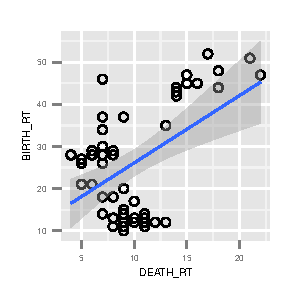
\includegraphics[width=2.25in,height=2.25in]{images/DEATH_RT-BIRTH_RT.pdf}
  \caption{Original interesting bivariate relationship}
 \label{fig:original2}
\end{figure}

\subsubsection{Divergence}

A Split that reveals unexpected or different structure than that seen in the original view adds to the user's understanding of the dataset. Different visual patterns function as an indicator of the conditioning dimension's importance in explaining some of the hidden structure in the data relationship being studied and its independence relative to the response dimensions being studied.

%Another visual pattern measure could be to use the correlation or slopes from linear regression fits to help distinguish splits where subsets of the data determined by the Partitioner dimension have particular linear relationships. This could help in the discovery of confounding covariates, the unexamined fields that have an effect on the data pattern. Simpson's paradox is a classic example of such mix-effects when aggregate numbers are affected by changes in the relative size and value of the subpopulations. 

To examine the divergence criterion we investigate whether our approach can pick out ``confounding variates" such as those that cause Simpson's Paradox. The Ourworld dataset of UN statistics on world countries~\cite{Wilkinson2005GG,Wilkinson2008} has such a known relationship when considering the positive correlation between the variables Death\_Rate and Birth\_Rate as seen in Figure~\ref{fig:original2}. We seek to reveal the visual structure by conditioning on variables in the dataset. Of the six categorical variables in the dataset, the one with the largest score using the $R^2$ metric for the goodness of linear fit is the GNP seen in Figure~\ref{fig:r2}. This Partitioner variable pulls apart the group of points/countries negatively correlated in the ``D" category from the strongly positively correlated set of countries in the ``U" category. Also, we see that when we have a small number of points in a split (category $0$), the distribution of scores from random samples is wide and flat as it is easy to infer patterns with a few points but these have low support.
\begin{figure}
\raggedleft
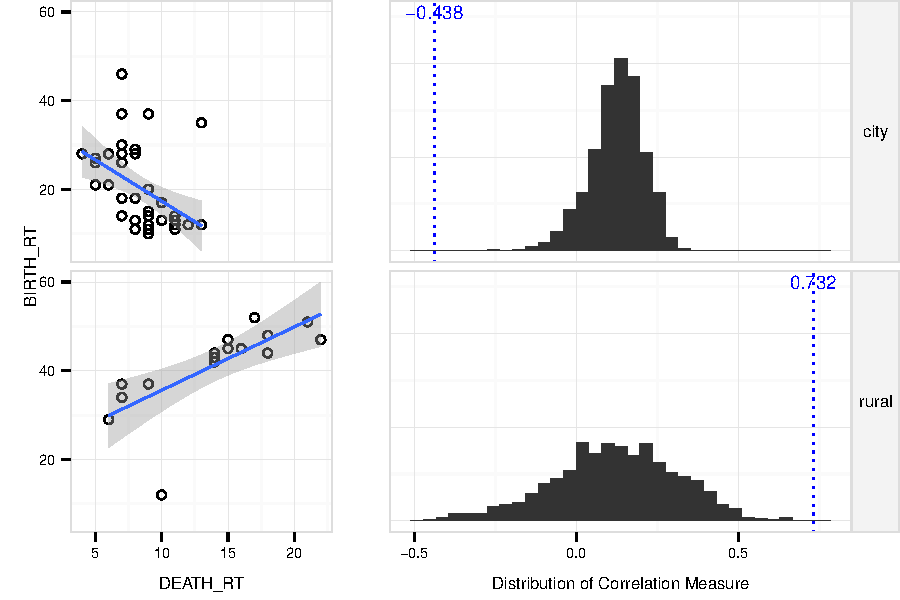
\includegraphics[width=3.5in,height=3.5in]{images/6_84034106410344-URBAN.pdf}
  \caption{r2}
 \label{fig:r2}
\end{figure}

\subsubsection{Support}
We expect to be conservative in our assessment of interesting patterns for ones with low support or determined by a small number of points. We see this in another split of the Ourworld data from the earlier example. Figure~\ref{fig:r2-leader} shows another interesting conditioning of the original interesting bivariate relationship. The higher cardinality Partitioner variable ``Leader" produces small individual splits which can be seen to have wide score distributions. Also, the splits produced by ``Leader" are not highly significant except for the ``Marxist" category.

%Risk Factors Associated with Low Infant Birth Weight~\cite{Hosmer1989}
\begin{figure}
\raggedleft
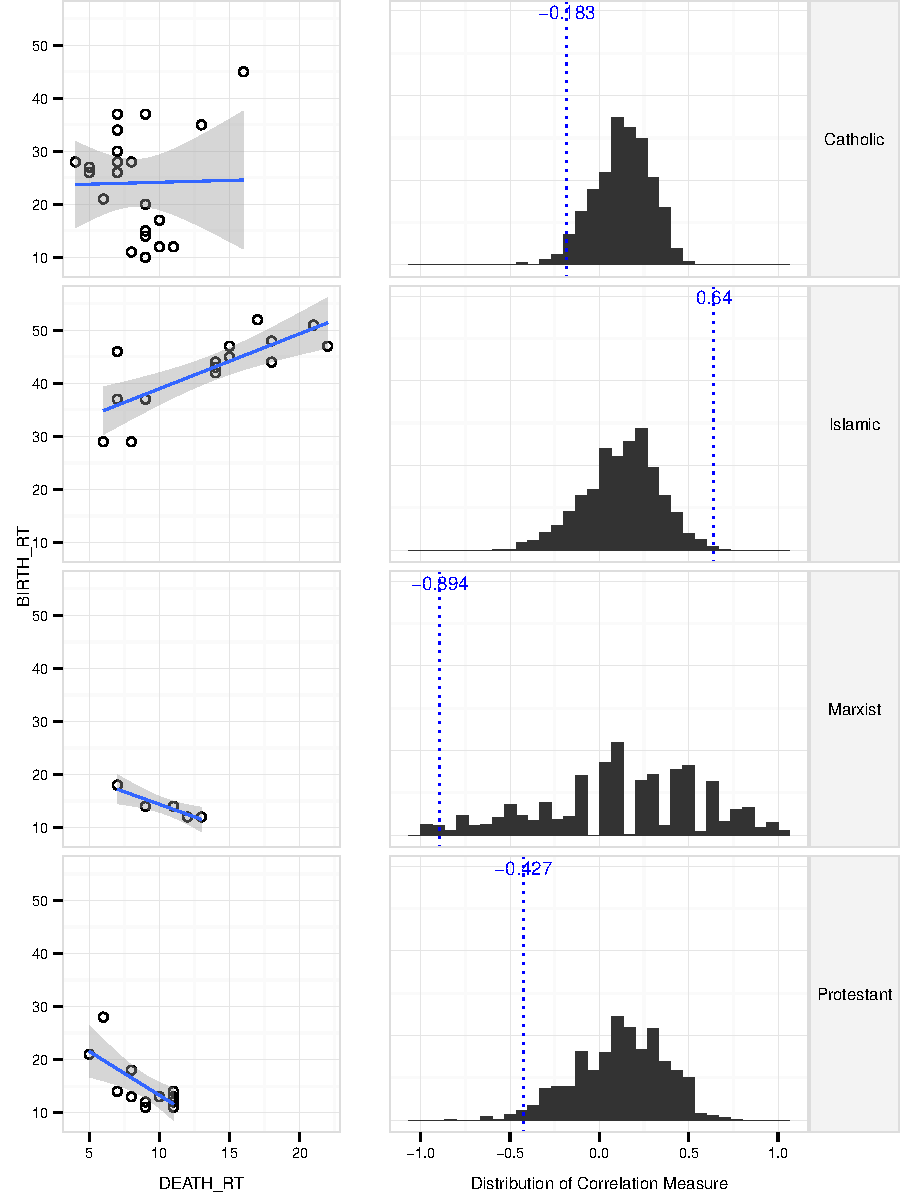
\includegraphics[width=3.5in,height=3.5in]{images/2_48595929670884-LEADER.pdf}
  \caption{r2}
 \label{fig:r2-leader}
\end{figure}

\subsubsection{Parsimonious}
High-cardinality Partitioners create a large number splits, which likely produce splits with low support as the observations get distributed among more facets. Not happy with this SuperStore example...

\subsubsection{Non-redundannt}
Discuss the weakness of our approach here.


\section{Discussion}
\label{sec:discussion}
Our approach of selecting Partitioner variables that showcase interesting visual explanations is generalizable in terms of allowing for a diversity of measures used to capture ``interesting visual structure". The wide range of measures surveyed~\cite{Bertini2011} can be used w/ our method based on the plot type of interest to describe the visual pattern of interest to find when partitioning a view.

When the parametric assumption (e.g. normal
distribution of data) is correct, the parametric
tests (z-, t-, F-tests) are more powerful.

Permutation test is more computationally
intensive


Furthermore, we can use this approach of selecting good splits of a data view to guide other multivariate exploratory data analysis applications.

Decision tree approach of guided EDA.

Trellis displays present a grid of plots of the same type showing the same variables conditioned on a Partitioner variable that determines the subsets of points shown in each plot. These displays are a very useful multivariate display as they are simple to interpret and provide an overview of large datasets for exploratory data analysis. Crucial to the layout of small multiples is the selection of a Partitioner variable to specify faceting into plots by rows and/or columns. This choice can then be repeated to facet the resulting plots further applying crossing and nesting.


